% Time-stamp: Aug  8 10:59 09intapps.tex
%!TEX root = free221.tex

% Add your name and the date here if you've done something.
% Evan, fixed batch of typos and some wording issues 12/23



\chapter{Applications of the integral}
The integral appears as the answer to many different questions.  In this chapter
we will describe a number of ``things that are an integral''.  In each example,
there is a quantity we want to compute which we can approximate through
Riemann sums.  After letting the partition become arbitrarily fine, we then find
that the quantity we are looking for is given by an integral.  The derivations
are an important part of the subject.

One could read this chapter as a list of formulas to compute areas, volumes,
lengths and other things, but that would be a mistake.  In each case the
important thing to learn is the reasoning that tells us how to turn a question
about areas, volumes, etc into an integral.

\section{Areas between graphs} %{{{1
% !!! Issue: Missing an example. Also missing a discussion of what happens if the curves cross.
\subsection{The problem} %{{{2
Suppose you have two functions $f$ and $g$ on an interval $[a,b]$ such that
$f(x)\leq g(x)$
for all $x$ in the interval $[a,b]$.  Then the area of the region between the
graphs of the two functions is
\begin{equation}
  \label{eq:area-between-graphs}
  \textrm{Area} = \int_a^b \bigl(g(x) - f(x) \bigr) dx.
\end{equation}
\begin{figure}[h]
  \leftline{ 
    \begin{picture} (150.000000,104.461538)(0,0)
    \put(0.0, 0.0){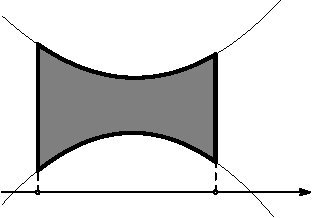
\includegraphics{09areabetweengraphs-setup.pdf}}
        \put( 16.08,   0.38){\sffamily\itshape $a$}
    \put(101.46,   0.38){\sffamily\itshape $b$}
    \put( 46.54,  73.81){\sffamily\itshape $y=g(x)$}
    \put( 46.54,  28.28){\sffamily\itshape $y=f(x)$}
\end{picture}

    
    \begin{picture} (150.000000,104.461538)(0,0)
    \put(0.0, 0.0){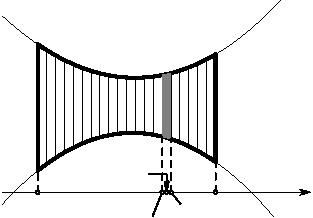
\includegraphics{09areabetweengraphs2.pdf}}
        \put( 16.08,   0.38){\sffamily\itshape $a$}
    \put(101.46,   0.38){\sffamily\itshape $b$}
    \put( 65.85,  -5.62){\sffamily\itshape $x_{k-1}$}
    \put( 81.85,   0.38){\sffamily\itshape $x_{k}$}
    \put( 62.90,  20.38){\sffamily\itshape $c_{k}$}
\end{picture}
 {\sffamily\footnotesize%
      \input ../figures/221/09area-between-graphs-one-slice.pdf_tex } }
  
  \caption{\textbf{The area between two graphs. } %
    To compute the area on the left you slice it into many thin vertical strips.
    Each strip is approximately a rectangle so its area is
    ``height$\times$width.''  }

\end{figure}
\subsection{Derivation using Riemann sums} %{{{2
To get this formula, we approximate the region by a large number of thin
rectangles.  Choose a partition $a=x_0<x_1<\cdots<x_n=b$ of the interval
$[a,b]$ and choose a number $c_k$ in each interval $[x_{k-1}, x_k]$. Then we form the
rectangles
\[
x_{k-1} \leq x\leq x_k,\qquad f(c_k)\leq y\leq g(c_k).
\]
The area of this rectangle is
\[
\text{width}\times\text{height} = \Delta x_k\cdot\bigl(g(c_k) - f(c_k)\bigr).
\]
Hence the combined area of the rectangles is
\[
R= \bigl(g(c_1) - f(c_1)\bigr)\Delta x_1 + \cdots + \bigl(g(c_n) -
f(c_n)\bigr)\Delta x_n
\]
which is just the Riemann sum for the integral on the right hand side in
\eqref{eq:area-between-graphs}.  Therefore,
\begin{itemize}

\item since the area of the region between the graphs of $f$ and $g$ is the
  limit of the combined areas of the rectangles,

\item and since this combined area is equal to the Riemann sum $R$,

\item and since the Riemann sums $R$ converge to the integral $I$,

\end{itemize}
we conclude that the area between the graphs of $f$ and $g$ is exactly the
integral in \eqref{eq:area-between-graphs}.

\subsection{Summary of the derivation} %{{{2
Since most applications of the integral follow the pattern in the derivation
above, it is important to understand its general features.
Here we can summarize the above calculation using Riemann sums by the following
(rather sketchy) argument: if we slice up the area between the two curves
$y=f(x)$ and $y=g(x)$ into $n$ strips all of width $\Delta x = \dfrac{b-a}{n}$,
then if we write the corresponding Riemann sum with $\Sigma$ notation, we have
\[
R= \sum_{j=1}^{n}\bigl(g(c_j) - f(c_j)\bigr)\Delta x.
\]
If we abuse the notation slightly and write the indices of summation as values
of $x$, this becomes
\[
R= \sum_{\text{``$x=a$''}}^{\text{``$x=b$''}}\bigl(g(x_j) - f(x_j)\bigr)\Delta x.
\]
Now, if we take the limit as $n \to \infty$, then the result is exactly the integral
\[
I= \int_{x=a}^{x=b}\bigl(g(x) - f(x)\bigr) \, dx.
\]
Essentially, the idea is that as we take the limit, the sum becomes an integral
and the ``$\Delta$''s become ``$d$''s.

\subsection{Leibniz' derivation} %{{{2
Many scientists and engineers think of integrals in terms of Leibniz's ``sums of
infinitely many infinitely small quantities,'' and will prefer the following
description of the derivation of the area formula \eqref{eq:area-between-graphs} 
\begin{quotation}
  \small\itshape \ldots
  to find the area of the region in the drawing on the right,
  divide this region into infinitely many infinitely
  thin strips.  Each strip has height $g(x) - f(x)$, where $x$ is the
  $x$-coordinate of the strip, and its width is the infinitely small number $dx$.
  \marginpar{ \footnotesize\sffamily\itshape%
  \input ../figures/221/09area-between-graphs-Leibniz.pdf_tex } The area of one of
  these strips is therefore
  \[
    \text{area of one infinitely thin strip} = \bigl(g(x) - f(x)\bigr) \times dx.
  \]
  To get the total area add the areas of all these infinitely
  thin strips together, which we (i.e. Leibniz) write as follows:
  \[
    \text{Area} =
    \mathop{\raisebox{-3pt}{\scalebox{0.8}[2.5]{\slshape\sffamily S}}}
    _{x=a}^{\;\;b} \bigl(g(x) - f(x)\bigr) dx.
  \]
\end{quotation}
The ``long s'' indicates that Leibniz is summing a lot of numbers.  This is
of course a very strange kind of sum, since the ``numbers'' he is adding are
infinitely small, and since there are infinitely many of them (there is one term
for each value of $x$ between $a$ and $b$!). Because there are infinitely many
terms in the sum you can't write it out using ``$+$''signs, and for this reason
Leibniz invented the notation we use for integration today.  The integral sign
is nothing but an elongated ``S'' and its shape should remind us that, at least
in Leibniz' interpretation, an integral comes about by adding infinitely many
infinitely small numbers.


\section{Problems} %{{{1
% !!! Issue: For the love of all that is whatever, can we get some
% areas-between-curves problems that AREN'T a line and a parabola?
\problemfont %{{{3
\begin{multicols}{2}\setlength{\parindent}{0pt}
\problem Find the area of the finite region bounded by the parabola $y^2=4x$ and %{{{3
the line $y=2x$.

\problem Find the area bounded by the curve $y=x(2-x)$ and the line $x=2y$. %{{{3

\problem Find the area bounded by the curve $x^2=4y$ and the line $x=4y-2$. %{{{3

\problem Calculate the area of the finite region bounded by the parabolas $y=x^2$ %{{{3
and $x=y^2$.

\problem Find the area of the finite region included between the parabola $y^2=x$ %{{{3
and the line $x+y=2$.

\problem Find the area of the finite region bounded by the curves $y=\sqrt{x}$ and %{{{3
$y=x$.

\problem Use integration to find the area of the triangular region bounded %{{{3
by the lines $y=2x+1$, $y=3x+1$ and $x=4$.


\problem Find the finite area bounded by the parabola $x^2-2=y$ and the line %{{{3
$x+y=0$.

\problem Where do the graphs of $f(x) = x^2$ and $g(x) = 3/(2+x^2)$ %{{{3
intersect?  Find the area of the region which lies above the graph of $y=f(x)$
and below the graph of $y=g(x)$.

(Hint: if you need to integrate $1/(2+x^2)$ you could substitute
$u=x/ \sqrt2$.)

\problem Graph the curve $y=(1/2)x^2+1$ and the straight line $y=x+1$ and %{{{3
find the area between the curve and the line.

\problem Find the area of the finite region between the parabolas $y^2=x$ and %{{{3
$x^2=16y$.

\problem Find the area of the finite region enclosed by the parabola $y^2=4ax$ and %{{{3
the line $y=mx$, where $a$ and $m$ are positive constants.

\problem Find $a$ so that the curves $y=x^2$ and $y=a\cos x$ intersect at %{{{3
the point $(x,y)=(\frac\pi4, \frac{\pi^2}{16})$. Then find the finite area
between these curves.

\problem \groupproblem Write a definite integral whose value is the %{{{3
area of the region between the two circles $x^2+y^2=1$ and
$(x-1)^2+y^2=1$.  Find this area.  [Hint: The area can be found using geometry,
using the observation that the part of a circle cut off by a line is a circular
sector with a triangle removed.]

\end{multicols}
\noproblemfont
\section{Cavalieri's principle and volumes of solids} %{{{1
In this section we'll discuss the ``method of slicing'' and use integration to
derive the formulas for volumes of spheres, cylinders, cones, and other solid
objects in a systematic way.

\subsection{Example -- Volume of a pyramid} %{{{2
As an example let's compute the volume of a pyramid whose base is a square of
side 1, and whose height is 1.  Our strategy will be to divide the pyramid into
thin horizontal slices whose volumes we can compute, and to add the volumes of
the slices to get the volume of the pyramid.

\begin{figure}[ht]
  \centering
  \parbox[b][80pt][t]{190pt}{\input ../figures/221/09pyramid2.tex }
  \hspace{35pt}
  \begin{minipage}[t]{130pt}
    \vbox to 80pt{\sffamily%
      \centerline{\bfseries\small Side view of the pyramid} \input ../figures/221/09pyramid2-sideview.pdf_tex } \vbox to
    80pt{\footnotesize\sffamily\itshape%
      A side view of the pyramid shows a triangle with base $1$ and height $1$.
      The slice at height $x$ cuts off a smaller triangle at the top.  The small
      and large triangles are similar.

      The height of the small triangle is $1-x$ times the height of the large
      triangle, so the base of the small triangle is $1-x$ times the base of the
      large triangle.  }
  \end{minipage}
  \caption{\textbf{Volume of a pyramid. } }
  \label{fig:09pyramid}
\end{figure}

To construct the slices we choose a partition of the (height) interval $[0, 1]$
into $N$ subintervals, i.e., we pick numbers
\[
0=x_0<x_1<x_2<\cdots<x_{N-1}<x_N=1,
\]
and as usual we set $\Delta x_k = x_k-x_{k-1}$.

The $k$th slice consists of those points on the pyramid whose height is between
$x_{k-1}$ and $x_k$.  The top of this slice is a square with side $1-x_k$ and
the bottom is a square with side $1-x_{k-1}$ (see Figure~\ref{fig:09pyramid}).
The height, or thickness, of the slice is $x_k-x_{k-1} = \Delta x_k$.

If you ignore the fact that the sides of the $k$th slice are slanted and not
vertical, then the volume of the $k$th slice is the product of the area of its
top and its thickness, i.e.  \marginpar{\footnotesize\sffamily\itshape%
  \input ../figures/221/09pyramid2-slice.pdf_tex}%
\[
\text{volume of $k$th slice} \approx (1-x_k)^2\Delta x_k.
\]
On the other hand, you could also estimate the volume of the slice by
multiplying the thickness and the area of the bottom instead of the top.  This
leads to
\[
\text{volume of $k$th slice} \approx (1-x_{k-1})^2\Delta x_k.
\]
Neither formula is exactly right and we might as well have chosen any $c_k$ in
the interval $[x_{k-1}, x_k]$ and estimated
\[
\text{volume of $k$th slice} \approx (1-c_k)^2\Delta x_k.
\]
The idea is that as we make the partition finer, each of these approximations
for the volume of a slice will get better, and that it won't matter which of
them we use.

Adding the volumes of the slices, we find that the volume $V$ of the pyramid is
given by
\[
V \approx (1-c_1)^2\Delta x_1 + \cdots + (1-c_N)^2\Delta x_N,
\]
where we expect the approximation to get better as we choose more and more
partition points.  The right hand side in this equation is a Riemann sum for the
integral
\[
I = \int_0^1 (1-x)^2dx
\]
and therefore we have
\[
I = \lim_{\cdots} \bigl\{ (1-c_1)^2\Delta x_1 + \cdots + (1-c_N)^2\Delta x_N
\bigr\} =V.
\]
Computing the integral then yields that the volume of the pyramid is
\[
V = \frac13.
\]

\subsection{Computing volumes by slicing -- the general case} %{{{2
The ``method of slicing,'' which we just used to compute the volume of a
pyramid, works for solids of any shape.  The strategy always consists of
dividing the solid into many thin (horizontal) slices, computing the volume of
each slice, summing the volumes of the slices, and then recognizing these sums
as Riemann sums for some integral.  That integral then is the volume of the
solid.

\begin{figure}[t]
  \centerline{
    \begin{picture} (270.000000,132.731707)(0,0)
    \put(0.0, 0.0){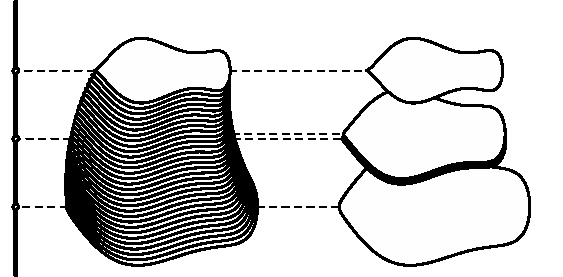
\includegraphics{09Xsections.pdf}}
        \put( -2.46,  31.68){\sffamily\itshape $a$}
    \put( -2.46,  64.37){\sffamily\itshape $x$}
    \put( -2.46,  97.05){\sffamily\itshape $b$}
    \put(244.85,  62.37){\sffamily\itshape Slice at height $x$}
    \put(179.63,  64.54){\sffamily\itshape Area $= A(x)$}
\end{picture}
}
  \caption{\textbf{Slicing a solid to compute its volume.}  The volume of one
    slice is approximately the product of its thickness ($\Delta x$) and the
    area $A(x)$ of its top.  Summing the volume $A(x)\Delta x$ over all slices
    leads approximately to the integral $\int_a^b A(x) dx$ (see
    \eqref{eq:09volume-by-slicing}.)}
  \label{fig:09Xslices}
\end{figure}

To be more precise, let $a$ and $b$ be the heights of the lowest and highest
points on the solid, and let $a=x_0<x_1<x_2<\ldots<x_{N-1}<x_N=b$ be a partition
of the interval $[a, b]$.  Such a partition divides the solid into $N$ distinct
slices, where slice number $k$ consists of all points in the solid whose height
is between $x_{k-1}$ and $x_k$.  The thickness of the $k$th slice is $\Delta x_k
= x_k-x_{k-1}$.  If
\[
A(x) = \text{area of the intersection of the solid with the plane at height
  $x$.}
\]
then we can approximate the volume of the $k$th slice by
\[
A(c_k) \Delta x_k
\]
where $c_k$ is any number (height) between $x_{k-1}$ and $x_k$.

The total volume of all slices is therefore approximately
\[
V\approx A(c_1)\Delta x_1 + \cdots + A(c_N)\Delta x_N.
\]
While this formula only holds approximately, we expect the approximation to get
better as we make the partition finer, and thus
\begin{equation}
  \label{eq:09vol-of-all-slices}
  V = \lim_{\cdots} \bigl(A(c_1)\Delta x_1 + \cdots + A(c_N)\Delta x_N\bigr).
\end{equation}
On the other hand the sum on the right is a Riemann sum for the integral $I=
\int_a^b A(x) dx$, so the limit is exactly this integral.  Therefore we have
\begin{equation}\label{eq:09volume-by-slicing}
  V = \int_a^b A(x)dx.
\end{equation}

In summary, to compute the volume of a solid, we pick an axis, slice up the solid perpendicular to that axis, and then integrate (along the axis) the cross-sectional areas of each of the slices.


\subsection{Cavalieri's principle} %{{{2
\begin{figure}[b]
  \centerline{
    \begin{picture} (180.000000,88.829268)(0,0)
    \put(0.0, 0.0){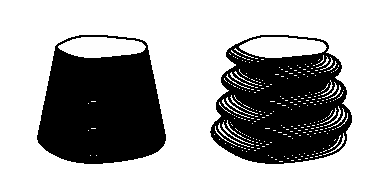
\includegraphics{09Cavalieri.pdf}}
    \end{picture}
}

  \caption{\textbf{Cavalieri's principle. }  Both solids consist of a pile of
    horizontal slices. The solid on the right was obtained from the solid on the
    left by sliding some of the slices to the left and others to the right.
    This operation does not affect the volumes of the slices, and hence both
    solids have the same volume.}
\end{figure}
The formula \eqref{eq:09volume-by-slicing} for the volume of a solid which we
have just derived shows that the volume only depends on the areas $A(x)$ of the
cross sections of the solid, and not on the particular shape these cross
sections may have.  This observation is older than calculus itself and goes back
at least to Bonaventura Cavalieri (1598 -- 1647) who said: {\itshape if the
  intersections of two solids with a horizontal plane always have the same area,
  no matter what the height of the horizontal plane may be, then the two solids
  have the same volume.  }

This principle is often illustrated by considering a stack of coins: If you put
a number of coins on top of each other then the total volume of the coins is
just the sum of the volumes of the coins.  If you change the shape of the pile
by sliding the coins horizontally then the volume of the pile will still be the
sum of the volumes of the coins, meaning that it doesn't change.
\subsection{Solids of revolution} %{{{2
In principle, formula \eqref{eq:09volume-by-slicing} allows you to compute the
volume of any solid, provided you can compute the areas $A(x)$ of all cross
sections.  One class of solids for which the areas of the cross sections are
easy are the so-called \emph{solids of revolution.}

\begin{figure}[h]\centering
  \parbox{175pt}{\input ../figures/221/09surf-of-rotation-profile.tex }
  \parbox{175pt}{\input ../figures/221/09surf-of-rotation21.tex }
  \parbox{175pt}{\input ../figures/221/09surf-of-rotation2.tex }
  \caption{\textbf{A solid of revolution} consists of all points in
    three-dimensional space whose distance $r$ to the $x$-axis satisfies $r\leq
    f(x)$.}
  \label{fig:09surf_of_rotation}
\end{figure}

A solid of revolution is created by rotating (revolving) the graph of a positive
function around the $x$-axis.  More precisely, let $f$ be a function that is
defined on an interval $[a, b]$ and that is always positive ($f(x)>0$ for all
$x$).  If you now imagine the $x$-axis floating in three dimensional space, then
\emph{the solid of revolution obtained by rotating the graph of $f$ around the
  $x$-axis} consists of all points in three-dimensional space with $a\leq x\leq
b$, and whose distance to the $x$-axis is no more than $f(x)$.

Yet another way of describing the solid of revolution is to say that the solid
is the union of all discs with centers $(x,0)$ that meet the $x$-axis perpendicularly and whose
radius is given by $r=f(x)$.

If we slice the solid with planes perpendicular to the $x$-axis, then
\eqref{eq:09volume-by-slicing} tells us the volume of the solid.  Each slice is
a disc of radius $r=f(x)$ so that its area is $A(x) = \pi r^2 = \pi f(x)^2$. We
therefore find that
\begin{equation}
  \label{eq:09volume_surf_of_revolution}
  V = \pi \int_a^b r^2 \; dx = \pi \int_a^b f(x)^2 \; dx.
\end{equation}

\subsection{Volume of a sphere} %{{{2
\label{sec:volume-sphere}
As an example we compute the volume of a sphere with radius $R$.  You can get
that sphere by revolving a semicircle with radius $R$ around the $x$-axis: this gives 
$r(x)=\sqrt{R^2-x^2}$.  Here is a drawing (don't get confused
by the fact that the $x$-axis is vertical in this picture):

\begin{figure}[h]\centering
  \input ../figures/221/09sliced-sphere.pdf_tex
  \caption{\textbf{On the left:} a sphere of radius $R$ with a slice of
    thickness $\Delta x$ at height $x$. \textbf{On the right:} a cross section
    which allows you to compute how the radius $r$ depends on $x$.}
\end{figure}
Since $r=\sqrt{R^2-x^2}$ we see that the area of a slice at height $x$ is
\[
A(x) = \pi r^2 =\Bigl(\sqrt{R^2-x^2}\Bigr)^2 = \pi \bigl(R^2-x^2\bigr).
\]
Furthermore, we only get slices if $-R \leq x \leq +R$, so the $x$ coordinate ranges
between $-R$ and $+R$.  The volume is therefore
\[
V = \pi \int_{-R}^R \bigl(R^2-x^2\bigr) \,dx =\pi \bigl[R^2x - \tfrac13
x^3\bigr]_{-R}^R =\tfrac{4} {3}\pi R^3,
\]
which is the standard formula we have seen before.



\subsection{Volume of a solid with a core removed -- the method of ``washers.''} %{{{2
\label{sec:volume-solid-with-core-removed}
Another class of solids whose volume you can compute by slicing arises when you
have one solid of revolution, and remove a smaller solid of revolution.  Here
we'll derive the formula for the volume.

\begin{figure}[ht]\centering
  \parbox{175pt}{\input ../figures/221/09surf-of-rotation3-profile.tex }
  \parbox{175pt}{\footnotesize\input ../figures/221/09surf-of-rotation3.tex }
  \caption{\textbf{The method of washers.}  If you remove one smaller solid of
    revolution from a larger solid of revolution you get the region that
    consists of all points in three-dimensional space whose distance $r$ to the
    $x$-axis satisfies $r_{\rm in} \leq r\leq r_{\rm out}$.  A thin slice of
    this solid looks like a washer.  }
  \label{fig:09method-of-washers}
\end{figure}

If the two solids have the same axis of rotation, and if the outer solid has
radius $r= r_{\rm out}=f(x)$, while the inner solid has radius $r=r_{\rm in} =
g(x)$, then the slice you get by intersecting the solid with a plane
perpendicular to the $x$-axis looks like a ``washer,'' or an \emph{annulus}
(ring shaped region).  The area of each ``infinitely thin'' slice is the
difference between the areas enclosed by the outer circle and the inner circle,
thus,
\[
A(x) = \pi r_{\rm out}(x)^2 - \pi r_{\rm in}(x)^2.
\]
The volume of such a slice is the product of its area $A(x)$ and its infinitely
small thickness~$dx$.  ``Adding'' the volumes of the thin washers together we
arrive at
\begin{equation}
  \label{eq:09volume-washers}
  V = \pi \int_a^b \bigl(r_{\rm out}(x)^2 -r_{\rm in}(x)^2\bigr)\; dx .
\end{equation}



\section{Three examples of volume computations of solids of revolution} %{{{1

\subsection{Problem 1: Revolve $\setR$ around the $y$-axis} %{{{2
\label{sec:09revolver-example1}
Consider the solid obtained by revolving the region
\[
\setR = \bigl\{ (x, y) \mid 0\leq x\leq 2, \quad (x-1)^2\leq y\leq 1\bigr\}
\]
around the $y$-axis.



\begin{figure}[hbt]
  \centering \rule[8pt]{\textwidth}{1pt}
  \begin{minipage}[b]{130pt}
    \vbox to 288pt{\footnotesize\sffamily%
      \textbf{Problem 1: } Computing the volume of the solid you get when you
      revolve this region around the $y$-axis.

      \smallskip

      \centerline{ 
    \begin{picture} (90.000000,54.800000)(0,0)
    \put(0.0, 0.0){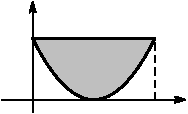
\includegraphics{09bowlregion.pdf}}
        \put(  8.67,  34.20){\sffamily\itshape 1}
    \put( 43.00,  -3.13){\sffamily\itshape 1}
    \put( 72.33,  -3.13){\sffamily\itshape 2}
    \put( 44.00,  19.53){\sffamily\itshape $\setR$}
\end{picture}
 }

      \smallskip

      The solid you get, with its top removed so you can look inside, and with a
      few cross sections (rotated copies of the region $\setR$) looks like this:
      \vfill

    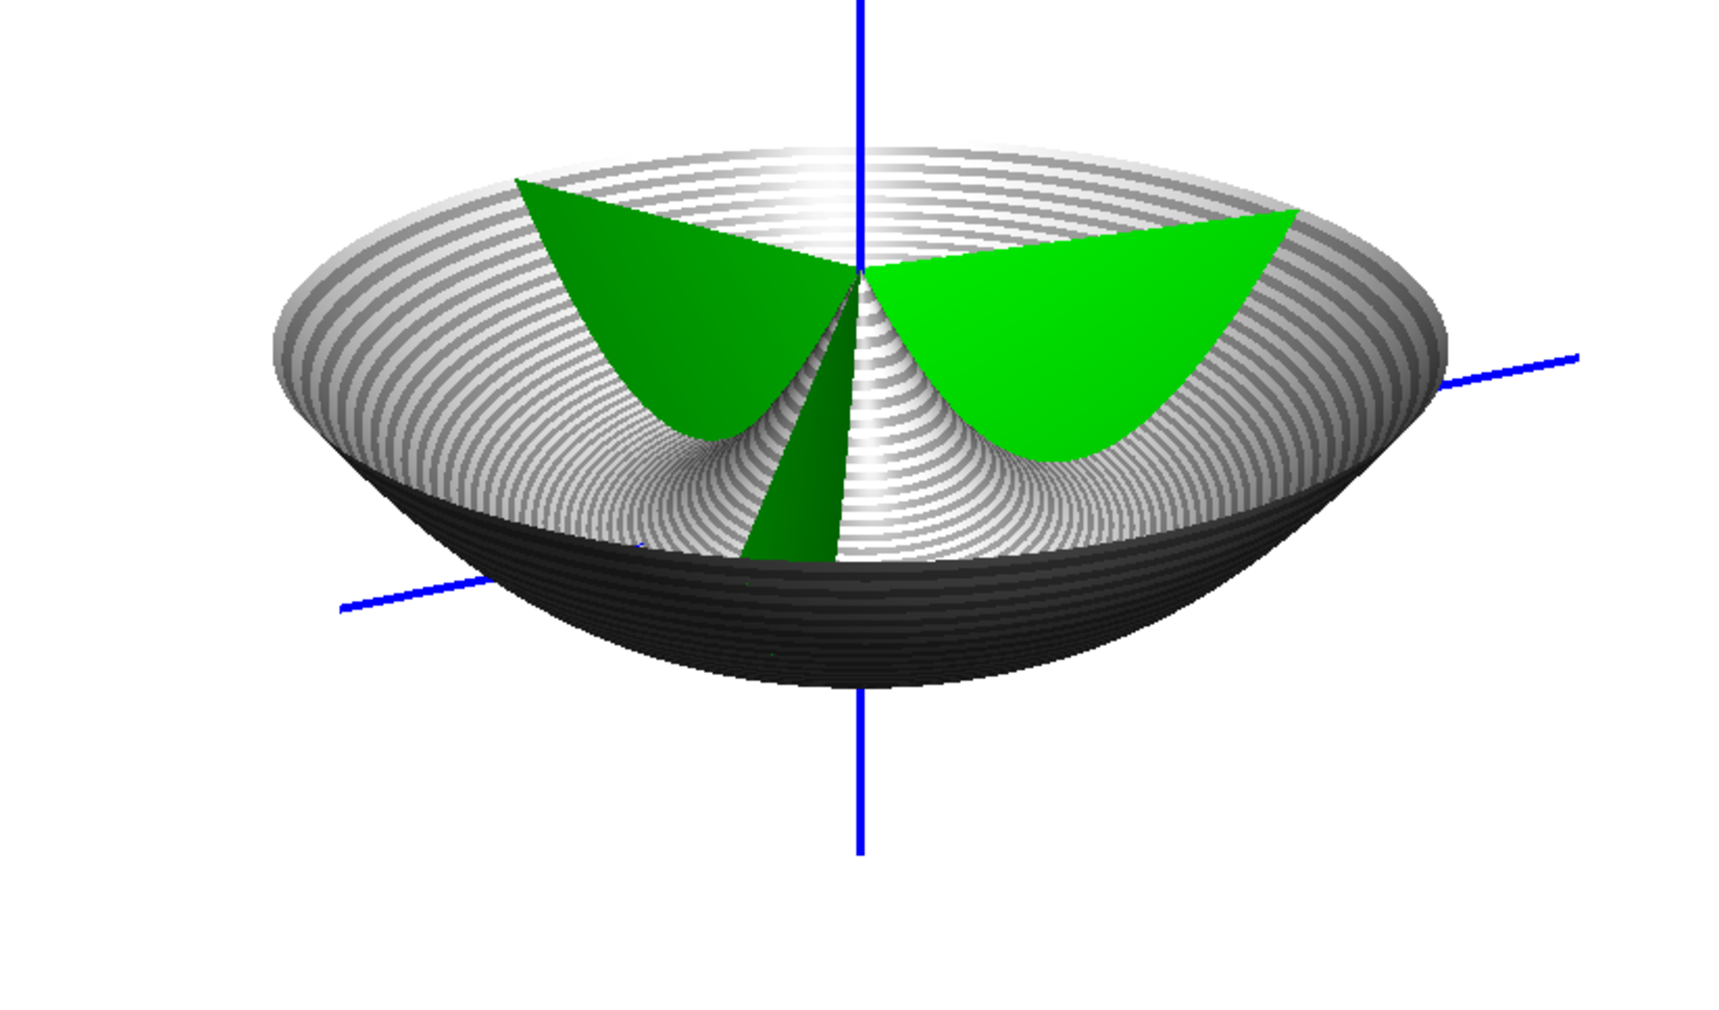
\includegraphics[width=125pt]{09surface-of-rotation1.pdf}
    \vfill

    On the right you see the drawing that is used in the computation of the
    volume. At the top is the cross section again.  When you rotate the line
    segment $AB$ around the $y$-axis it sweeps out a ``washer,'' pictured below.
  }
\end{minipage}%\;\vrule\;
\begin{minipage}[b]{220pt}
  \input ../figures/221/09bowl.tex
\end{minipage}
\rule{\textwidth}{1pt}

\end{figure}


\textbf{Solution: } The region we have to revolve around the $y$-axis consists
of all points above the parabola $y=(x-1)^2$ but below the line $y=1$.

If we intersect the solid with a plane at height $y$ then we get a ring shaped
region, or ``annulus'', i.e.\ a large disc with a smaller disc removed.  You can
see it in the figure below: if you cut the region $\setR$ horizontally at height
$y$ you get the line segment $AB$, and if you rotate this segment around the
$y$-axis you get the grey ring region pictured below the graph.  Call the radius
of the outer circle $r_{\textrm{out}}$ and the radius of the inner circle
$r_{\textrm{in}}$.  These radii are the two solutions of
\[
y = (1-r)^2
\]
so they are
\[
r_{\textrm{in}} = 1-\sqrt y, \qquad r_{\textrm{out}} = 1+\sqrt y.
\]
The area of the cross section is therefore given by
\[
A(y) = \pi r_{\textrm{out}}^2 - \pi r_{\textrm{in}}^2 =\pi\bigl(1+\sqrt{y}\bigr)^2 - \pi\bigl(1-\sqrt{y}\bigr)^2 =4\pi\sqrt{y}.
\]
The $y$-values which occur in the solid are $0\leq y\leq 1$ and hence the volume
of the solid is given by
\[
V = \int_0^1 A(y) dy = 4\pi \int_0^1\sqrt y\; dy = 4\pi \cdot \tfrac23 =
\frac{8\pi}3.
\]

\subsection{Problem 2: Revolve $\setR$ around the line $x=-1$} %{{{2
Find the volume of the solid of revolution obtained by revolving the same region
$\setR$ around the line $x=-1$.

\textbf{Solution: } The line $x=-1$ is vertical, so we slice the solid with
horizontal planes.  The height of each plane will be called $y$.

\begin{figure}[hbt]
  \centering \rule[8pt]{\textwidth}{1pt}
  \begin{minipage}[b]{130pt}
    \vbox to 288pt{\footnotesize\sffamily%
      \centerline{ 
    \begin{picture} (90.000000,54.800000)(0,0)
    \put(0.0, 0.0){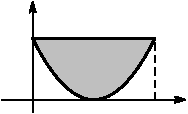
\includegraphics{09bowlregion.pdf}}
        \put(  8.67,  34.20){\sffamily\itshape 1}
    \put( 43.00,  -3.13){\sffamily\itshape 1}
    \put( 72.33,  -3.13){\sffamily\itshape 2}
    \put( 44.00,  19.53){\sffamily\itshape $\setR$}
\end{picture}
 }

      \smallskip

      \textbf{Problem 2: } In this problem we revolve the region $\setR$ around
      the line $x=-1$ instead of around the $y$-axis.

      The solid you get, again with its top removed so you can look inside, and
      with a few cross sections (rotated copies of the region $\setR$) looks
      like this: \vfill

    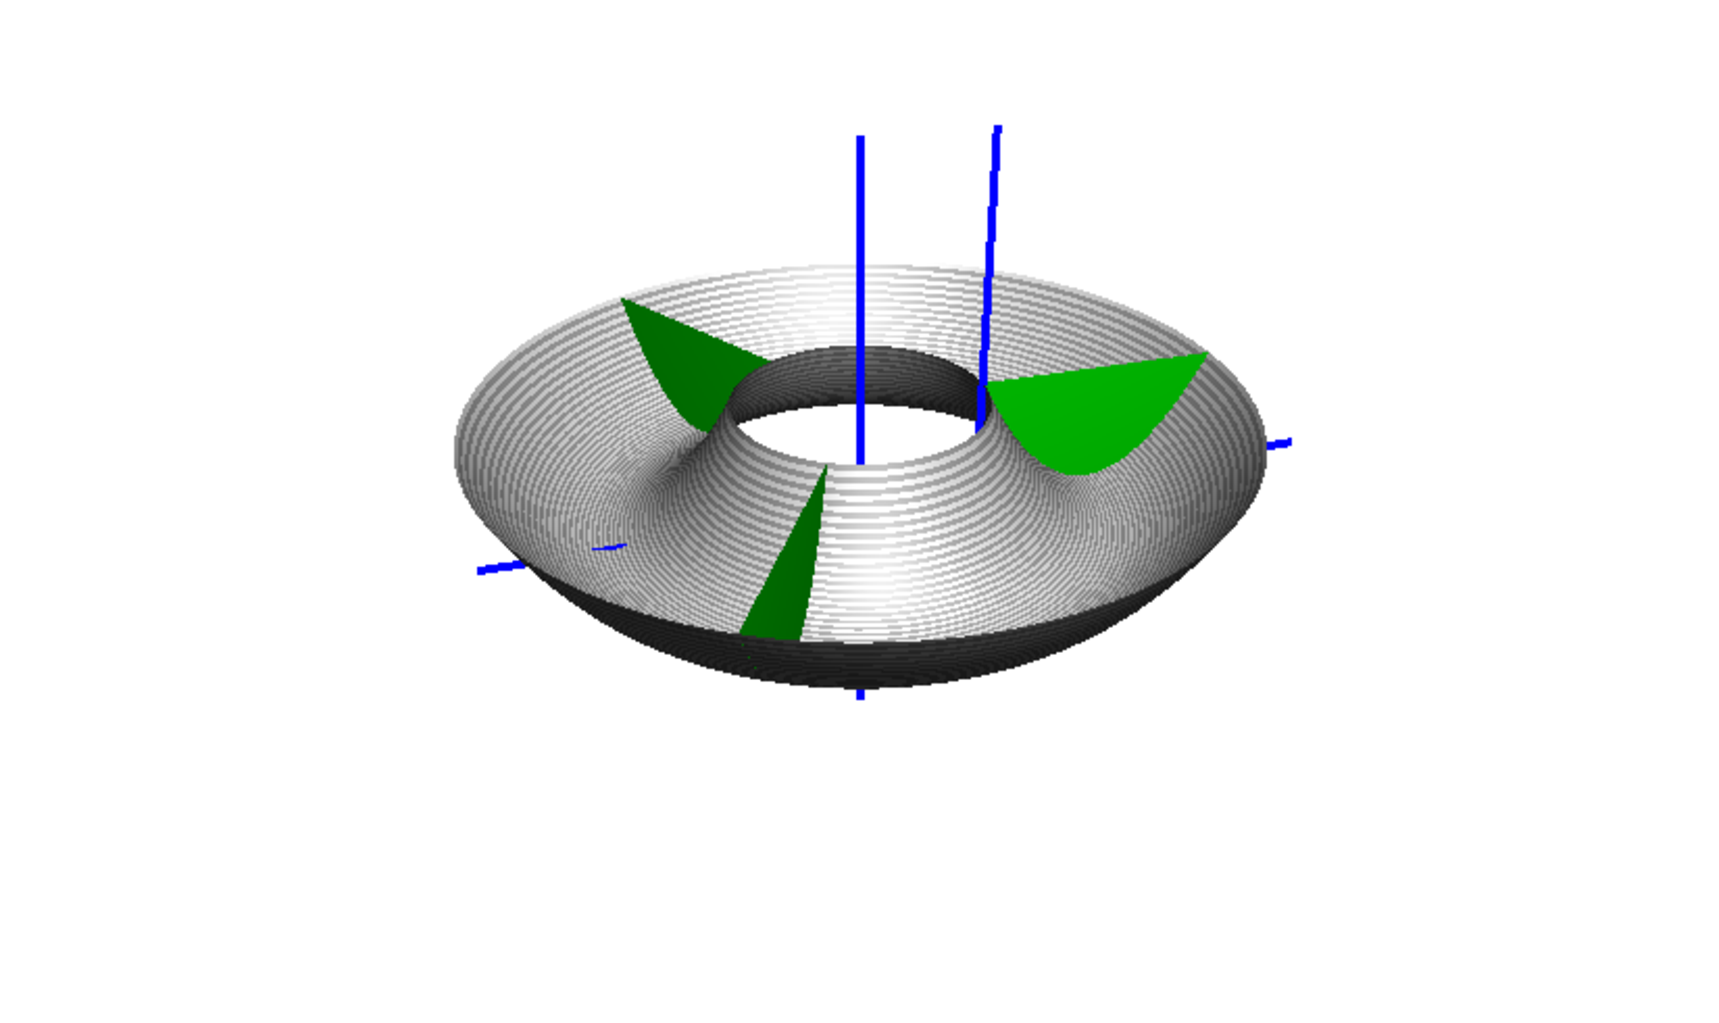
\includegraphics[width=125pt]{09surface-of-rotation2.pdf}
    \vfill

    On the right you see the drawing that is used in the computation of the
    volume, with the cross section again at the.  Rotating the line segment $AB$
    around the line $x=1$ produces the ``washer,'' pictured below.  }
\end{minipage}%\;\vrule\;
\begin{minipage}[b]{220pt}
  \sffamily\centering 
    \begin{picture} (220.000000,263.600000)(0,0)
    \put(0.0, 0.0){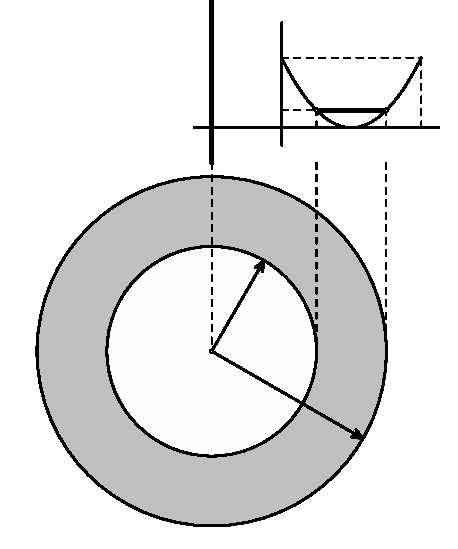
\includegraphics{09bowl_variation1.pdf}}
        \put(190.23, 239.77){\sffamily\itshape $y=(x-1)^2$}
    \put(151.92, 214.62){\sffamily\itshape $A$}
    \put(181.46, 214.62){\sffamily\itshape $B$}
    \put(149.92, 192.23){\sffamily\itshape $x_{\mathrm{in}}$}
    \put(116.19, 110.69){\sffamily\itshape $r_{\mathrm{in}}$}
    \put(183.46, 192.23){\sffamily\itshape $x_{\mathrm{out}}$}
    \put(152.66,  70.06){\sffamily\itshape $r_{\mathrm{out}}$}
    \put(212.29, 202.23){\sffamily\itshape $x$}
    \put(128.15, 234.77){\sffamily\itshape 1}
    \put(166.69, 192.23){\sffamily\itshape 1}
    \put(200.23, 192.23){\sffamily\itshape 2}
    \put(128.15, 209.62){\sffamily\itshape $y$}
    \put(101.62,  28.07){\sffamily\itshape \makebox[0pt][c]{Area$=\pi r_{\rm out}^2-\pi r_{\rm in}^2$}}
    \put( 92.62, 205.23){\sffamily\itshape \rotatebox{90}{Rotation axis}}
    \put( 34.54, 235.77){\sffamily\itshape SIDE VIEW:}
    \put( 34.54, 185.46){\sffamily\itshape TOP VIEW:}
\end{picture}

\end{minipage}
\rule{\textwidth}{1pt}

\end{figure}
As before the slices are ring shaped regions (``washers'') but the inner and
outer radii are now given by
\[
r_{\textrm{in}} = 1+x_{\textrm{in}} = 2-\sqrt y,\qquad r_{\textrm{out}} =
1+x_{\textrm{out}} = 2+\sqrt y.
\]
The volume is therefore given by
\[
V=\int_0^1 \bigl(\pi r_{\textrm{out}}^2-\pi r_{\textrm{in}}^2\bigr)dy
=\pi\int_0^1 8\sqrt y\; dy =\frac{16\pi}3.
\]


\subsection{Problem 3: Revolve $\setR$ around the line $y=2$} %{{{2
Compute the volume of the solid you get when you revolve the same region $\setR$
around the line $y=2$.

\begin{figure}[h]
  \rule{\textwidth}{1pt} \sffamily\centering
  
    \begin{picture} (270.000000,174.285714)(0,0)
    \put(0.0, 0.0){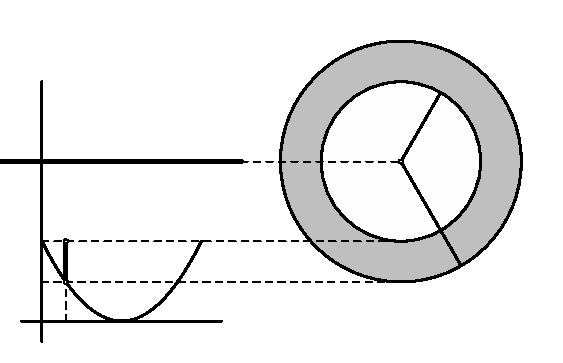
\includegraphics{09bowl_variation2.pdf}}
        \put( 58.43, 100.71){\sffamily\itshape Rotation axis}
    \put( 33.63,  42.90){\sffamily\itshape $A$}
    \put( 27.63,  62.43){\sffamily\itshape $B$}
    \put( 29.63,  10.14){\sffamily\itshape $x$}
    \put(208.88, 115.75){\sffamily\itshape $r_{\mathrm{in}}$}
    \put(205.91,  78.82){\sffamily\itshape $r_{\mathrm{out}}$}
    \put(-15.86,  37.90){\sffamily\itshape $(1-x)^2$}
    \put( 13.14,  57.43){\sffamily\itshape 1}
    \put( 13.14, 100.71){\sffamily\itshape 2}
    \put( 56.43,  10.14){\sffamily\itshape 1}
    \put( 94.71,  10.14){\sffamily\itshape 2}
    \put(157.97,  27.80){\sffamily\itshape Area$=\pi r_{\mathrm{out}}^2-\pi r_{\mathrm{in}}^2$}
\end{picture}


      \parbox{144pt}{ \vbox to 120pt{
          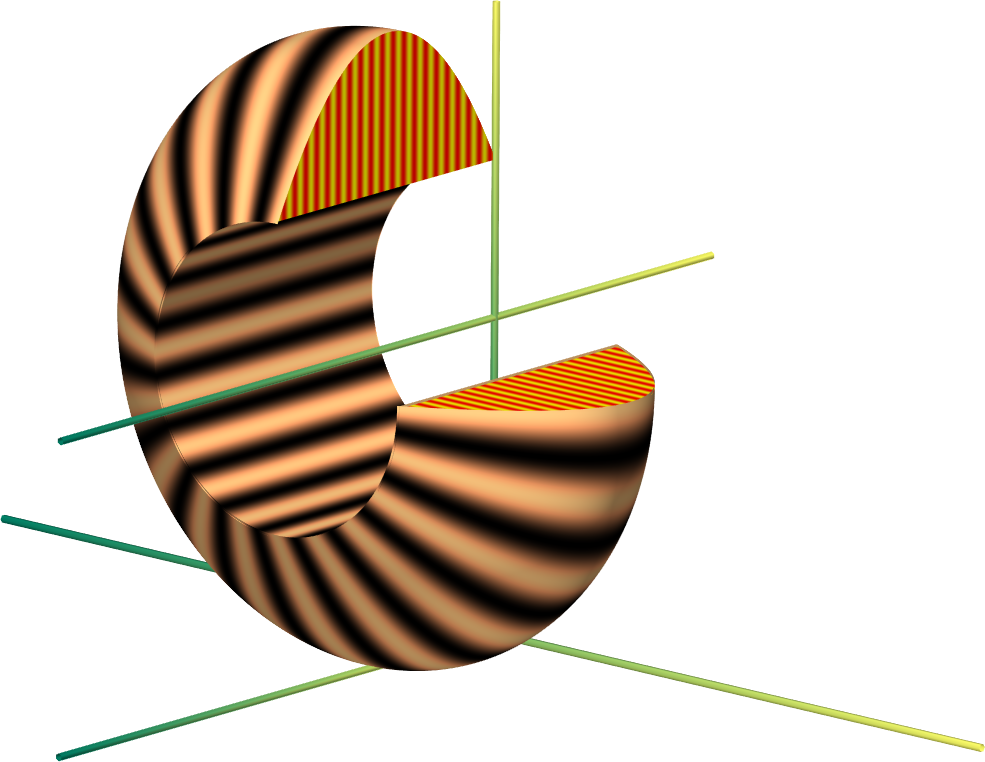
\includegraphics[width=144pt]{09ring.png}} } \qquad
      \parbox{130pt}{\vbox to 120pt{\footnotesize\sffamily%
      \textbf{Problem 3:} We revolve the same region $\setR$ as in the previous
      two problems about the line $y=2$.  The solid you get is shown on the left
      (cut open to show that the cross section is the region $\setR$).
      
      Above is the drawing that is used to find the inner and outer radii of 
      the washers you get when you rotate the line segment $AB$ around the
      horizontal line $y=2$.}}  \rule{\textwidth}{1pt}
      
\end{figure}

\textbf{Solution: } This time the line around which we rotate $\setR$ is
horizontal, so we slice the solid with planes perpendicular to the $x$-axis.

A typical slice is obtained by revolving the line segment $AB$ about the line
$y=2$.  The result is again an annulus, and from the figure we see that the
inner and outer radii of the annulus are
\[
r_{\textrm{in}} = 1,\qquad r_{\textrm{out}} = 2-(1-x)^2.
\]
The area of the slice is therefore
\[
A(x) = \pi \bigl(2-(1-x)^2\bigr)^2-\pi \cdot 1^2 = \pi\left( 3-4(1-x)^2+(1-x)^4
\right).
\]
The $x$ values which occur in the solid are $0\leq x\leq2$, and so its volume is
\begin{align*}
  V &= \pi\int_0^2\left( 3-4(1-x)^2+(1-x)^4 \right)dx\\
  &=\pi\left[ 3x+\tfrac43(1-x)^3-\tfrac15(1-x)^5 \right|_0^2\\
  &=\tfrac{56}{15}\pi
\end{align*}

\newpage% Need to force a new page to get the cylindrical shell
        % picture in the right place
\section{Volumes by cylindrical shells}
\vbox to 0pt{\hsize130pt\centering%
  
    \begin{picture} (120.000000,161.647059)(0,0)
    \put(0.0, 0.0){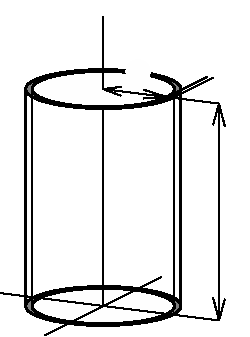
\includegraphics{09cylindricalSHELL.pdf}}
        \put(107.12,  60.00){\sffamily\itshape $h$}
    \put( 62.69, 119.61){\sffamily\itshape $r$}
    \put( 97.56, 126.90){\sffamily\itshape $\Delta r$}
\end{picture}


  \footnotesize\sffamily\itshape Finding the volume of a\\
  thin cylindrical shell } \hangindent140pt\hangafter-17 Instead of slicing a
solid with parallel planes you can also compute its volume by splitting it into
thin cylindrical shells and adding the volumes of those shells.  To find the
volume of a thin cylindrical shell, recall that the volume of a cylinder of
height $h$ and radius $r$ is $\pi r^2h$ (height times the area of the base).  Therefore the
volume of a cylindrical shell of height $h$, (inner) radius $r$ and thickness
$\Delta r$ is
\[\displayindent140pt \displaywidth220pt
\begin{array}{rcl}
  \pi h(r+\Delta r)^2 - \pi hr^2
  &=&\pi h (2r+\Delta r) \Delta r\\
  &\approx& 2\pi h r \Delta r.
\end{array}
\]
Now consider the solid you get by revolving the region
\[\displayindent140pt \displaywidth220pt
\setR = \left\{ (r, h) \mid a\leq r\leq b, 0\leq h\leq f(r) \right\}
\]
around the $h$-axis (instead of using $x$ and $y$ we put $r$ on the horizontal
axis and $h$ on the vertical axis as in Figure~\ref{fig:09cylindricalshells}).
By partitioning the interval $a\leq r \leq b$ into many small intervals we can
decompose the solid into many thin shells.  The volume of each shell will
approximately be given by $2\pi rf(r)\Delta r$.  Adding the volumes of the
shells, and taking the limit over finer and finer partitions we arrive at the
following formula for the volume of the solid of revolution:
\begin{equation}
  V = 2\pi\int_a^b rf(r) \;dr.
\end{equation}


\begin{figure}[t]\centering
  
  \parbox{175pt}{
    \begin{picture} (150.000000,113.000000)(0,0)
    \put(0.0, 0.0){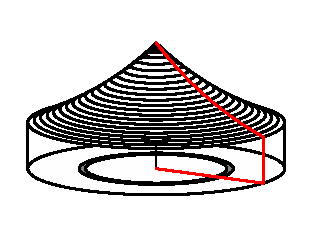
\includegraphics{09solidWITHmanyshells.pdf}}
    \end{picture}
 }
  \parbox{175pt}{
    \begin{picture} (150.000000,113.000000)(0,0)
    \put(0.0, 0.0){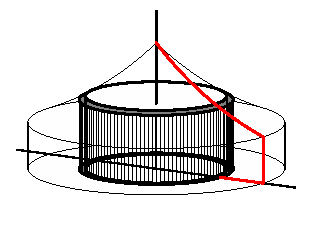
\includegraphics{09solidWITHshells.pdf}}
        \put(143.57,  21.47){\sffamily\itshape $r$}
    \put( 77.00, 104.28){\sffamily\itshape $h$}
\end{picture}
 }
  
  \caption{Computing the volume under a circus tent using cylindrical shells.
    This particular tent is obtained by rotating the graph of $y=e^{-x}$, $0\le
    x\le 1$ around the $y$-axis.}
  \label{fig:09cylindricalshells}
\end{figure}

If the region $\setR$ is not the region under the graph, but rather the region
between the graphs of two functions $f(r)\leq g(r)$, then we get
\[
V = 2\pi\int_a^b r\bigl(g(r) - f(r)\bigr) \;dr.
\]

\subsection{Example -- The solid obtained by rotating $\setR$ about the $y$-axis, again} %{{{2
The region $\setR$ from \S\ref{sec:09revolver-example1} can also be described as
\[
\setR = \bigl\{(x, y) \mid 0\leq x\leq 2, f(x)\leq y\leq g(x)\bigr\},
\]
where
\[
f(x) = (x-1)^2\text{ and }g(x) = 1.
\]
The volume of the solid which we already computed in
\S\ref{sec:09revolver-example1} is thus given by
\begin{align*}
  V &= 2\pi \int_0^1 x\bigl\{1-(x-1)^2\bigr\}\;dx\\
  % &= 2\pi\int_0^2 x\bigl\{1-x^2+2x-1\bigr\}\;dx \\
  &= 2\pi \int_0^2 \bigl\{-x^3+2x^2\bigr\}\;dx\\
  &= 2\pi\bigl[-\tfrac14x^4+\tfrac23x^3\bigr]_0^2\\
  % = 2 pi (-2^4/4 + 2/3 2^3) = 2 pi (-4 + 16/3) = 8 pi /3
  &= 8\pi/3,
\end{align*}
which coincides with the answer we found in \S\ref{sec:09revolver-example1}.




\section{Problems} %{{{1
\problemfont %{{{3
\begin{multicols}{2}\setlength{\parindent}{0pt}
\problem \groupproblem What do the dots in ``$\lim_{\cdots}$'' in equation %{{{3
\eqref{eq:09vol-of-all-slices} stand for? (In other words, what approaches what
in this limit?)
\[
\clubsuit
\]
\problem  %{{{3
Find the volume enclosed by the paraboloid obtained by rotating the
graph of $f(x) = R \sqrt{x/H}$ ($0\leq x\leq H$) around the $x$-axis.
Here $R$ and $H$ are positive constants.  Draw the solid whose volume
you are asked to compute, and indicate what $R$ and $H$ are in your
drawing.
\[
\heartsuit
\]
\begingroup\itshape
Find the volume of the solids you get by rotating each of the
following graphs around the $x$-axis:
\endgroup

\problem $f(x) = x$, $0\leq x\leq 2$  %{{{3

\problem $f(x) = \sqrt{2-x}$, $0\leq x\leq 2$  %{{{3

\problem $f(x) = \bigl(1+x^2\bigr)^{-1/2}$, $|x|\leq1$  %{{{3

\problem $f(x) = \sin x$, $0\leq x\leq \pi$  %{{{3

\problem $f(x) = 1-x^2$, $|x|\leq 1$  %{{{3

\problem $f(x) = \cos x$, $0\leq x\leq \pi$  [Note that this function crosses %{{{3
the $x$-axis: is this a problem?]

\problem $f(x) = 1/\cos x$, $0\leq x\leq \pi/4$  %{{{3

\problem  \label{ex:SphereVolume} %{{{3
Find the volume that results by rotating the semicircle
$y=\sqrt{R^2-x^2}$ about the $x$-axis, for $-R \leq x \leq R$.

\problem Let $\setT$ be the triangle $1\le x\le 2$, $0\le y\le 3x-3$. %{{{3
 
Find the volume of the solid obtained by \ldots

\subprob \ldots rotating $\setT$ around the $x$-axis.

\subprob \ldots rotating $\setT$ around the $y$ axis.

\subprob \ldots rotating $\setT$ around the line $x=-1$.

\subprob \ldots rotating $\setT$ around the line $y=-1$.



\problem A spherical bowl of radius $a$ contains water to a %{{{3
depth $h<2a$. 

\subprob  Find the volume of the water in the bowl in terms of $h$ and $a$.  (Which
solid of revolution is implied in this problem?)

\subprob  Water runs into a spherical bowl of radius 5 ft at
the rate of 0.2 ft${}^3$/sec. How fast is the water level rising
when the water is 4 ft deep?

\problem \label{ex:09archimedes} %{{{3
What we have called Cavalieri's principle was already known in some
form to Archimedes.  He used this idea to compute the volumes of
various solids.  One of his more famous discoveries is depicted below
in Figure \ref{fig:09archimedes-sphere-cone-cylinder}.  He found that
the ratios of the volumes of a cone of height and radius $R$,
half a sphere of radius $R$, and a cylinder of height and
radius $R$ are given by this very simple rule:
\[
  \textbf{cone}:
  \textbf{sphere}:
  \textbf{cylinder}
  =
  \textbf{1}:\textbf{2}:\textbf{3}
\]
In other words, the half sphere has twice the volume of the cone, and the
cylinder has three times the volume of the cone.

\subprob Prove Archimedes is right by computing the volumes of these solids
of revolution.  

\smallskip

This computation will give you practice in setting up and doing integrals, which
you compute by using a fair amount of algebra\footnote{In the time of Archimedes there were no integrals nor even algebra, so we might wonder: how did Archimedes do this? The answer is: a combination of his ``lever principle'' and a complicated geometric argument by contradiction showing that a cone has one-third the area of the cylinder with the same base and height}.

\carefulnow\subprob Show that the volume of the cone plus the volume of the half-sphere is
exactly the volume of the cylinder by comparing the areas of slices and using
Cavalieri's principle (and thus without doing any integrals).

\end{multicols}
\noproblemfont
\begin{figure}[h]
  \centering \input ../figures/221/09archimedes-sphere-cone-cylinder.pdf_tex
  \caption{\textbf{Archimedes' volume computation. }  See
    problem~\ref{ex:09archimedes}.}
  \label{fig:09archimedes-sphere-cone-cylinder}
\end{figure}

\section{Distance from velocity} %{{{1

\subsection{Motion along a line} %{{{2
If an object is moving on a straight line, and if its position at time $t$ is
$x(t)$, then we had defined the velocity to be $v(t) = x'(t)$.  Therefore the
position is an antiderivative of the velocity, and the fundamental theorem of
calculus says that
\begin{equation}
  \label{eq:distance-from-velocity}
  \int_{t_a}^{t_b} v(t)\;dt = x(t_b) - x(t_a),
\end{equation}
or
\[
x(t_b) = x(t_a) + \int_{t_a}^{t_b} v(t)\; dt.
\]
In words, the integral of the velocity gives you the distance travelled by the
object (during the interval of integration).

You can also get equation \eqref{eq:distance-from-velocity} by using Riemann
sums.
\begin{figure}[h]
  \begin{center}
    \def\svgwidth{240pt} \footnotesize \input ../figures/221/09cars.pdf_tex
  \end{center}
\end{figure}
Namely, to see how far the object moved between times $t_a$ and $t_b$ you choose
a partition $t_a=t_0<t_1<\cdots<t_N=t_b$.  Let $\Delta s_k$ be the distance
travelled during the time interval $(t_{k-1}, t_k)$.  The length of this time
interval is $\Delta t_k = t_k-t_{k-1}$.  During this time interval the velocity
$v(t)$ need not be constant, but if the time interval is short enough then you
can estimate the velocity by $v(c_k)$ where $c_k$ is some number between
$t_{k-1}$ and $t_k$.  You then have
\[
\Delta s_k \approx v(c_k) \Delta t_k
\]
Here the approximation will be more accurate as you make the $\Delta t_k$'s
smaller.  The total distance travelled is the sum of the travel distances for
all time intervals $t_{k-1}<t<t_k$, i.e.
\[
\text{Distance travelled} \approx \Delta s_1 +\cdots+\Delta s_N \approx
v(c_1)\Delta t_1 + \cdots + v(c_N)\Delta t_N.
\]
The right hand side is again a Riemann sum for the integral in
\eqref{eq:distance-from-velocity}.  As you make the partition finer and finer
you therefore get
\[
\text{Distance travelled} = \int_{t_a}^{t_b} v(t)\; dt.
\]
\textsc{Leibniz} would have said it even shorter:
\begin{quotation}\itshape
  \ldots to see how far the object travelled between time $t_a$ and time $t_b$,
  I, Leibniz, divide the interval $t_a < t < t_b$ into infinitely many
  intervals, each of length $dt$.  This length $dt$ has to be infinitely small.
  During the infinitely short time interval from $t$ to $t+dt$ the velocity is
  constant, so the distance travelled is $v(t)\,dt$.  When I ſum all these
  infinitely short displacements over all the time intervals I get
  \[
    \text{Diſtance travelled} =
    \mathop{\text{\Large ſ}}\limits_{t=t_a}^{t_b} v(t)\; dt.
  \]
\end{quotation}
Again, we have to wonder what ``adding infinitely many infinitely small
quantities'' actually means.  Leibniz never explained that.  Fortunately the
derivation with Riemann sums leads to the same answer.

\subsection{The return of the dummy} %{{{2
Often you want to write a formula for $x(t)=\cdots$ rather than $x(t_b)=\cdots$
as we did in \eqref{eq:distance-from-velocity}, i.e.\ you want to say what the
position is at time $t$, instead of at time $t_a$.  For instance, you might want
to express the fact that the position $x(t)$ is equal to the initial position
$x(0)$ plus the integral of the velocity from $0$ to $t$.  To do this you cannot
write
\[
\text{\carefulnow\carefulnow}\quad x(t) = x(0) + \int^{t}_{0} v(t)\; dt \quad
\boldmath{\longleftarrow} \quad \textbf{BAD FORMULA}
\quad\text{\carefulnow\carefulnow}
\]
because the variable $t$ gets used with two different meanings: the $t$ in
$x(t)$ on the left, and in the upper bound on the integral ($\int^t$) are the
same, but they are not the same as the two $t$'s in $v(t)dt$.  The latter is a
dummy variable (see Chapter~III, \S\ref{sec:free-versus-dummy-variables} and
Chapter~VIII, \S\ref{sec:08terminology}).  To fix this formula we should choose a different
letter or symbol for the integration variable.  A common choice in this
situation is to decorate the integration variable with a prime ( $t'$ ), a tilde
( $\tilde{t}$ ) or a bar ( $\bar t$ ).  So you can write
\[
x(t) = x(0) + \int^{t}_{0} v(\bar t)\; d\bar t.
\]

\subsection{Motion along a curve in the plane} %{{{2
If an object is moving in the plane, and if its position is given by
\[
x = x(t), \quad y = y(t)
\]
then we can also compute the distance travelled during any time interval.  The
derivation is very similar to the discussion of the velocity of a parametric
curve in Chapter V, \S\ref{sec:05parametrized-curves-and-lHopital}.

To find the distance travelled between $t=t_a$ and $t=t_b$, divide the time
interval into many short intervals
\[
t_a=t_0<t_1<\cdots<t_N=t_b.
\]
You then get a sequence of points
\[
P_0(x(t_0), y(t_0)),\; P_1(x(t_1), y(t_1)),\; \ldots,\; P_N(x(t_N), y(t_N)),
\]
and after ``connecting the dots'' you get a polygon.  You could approximate the
\begin{figure}[ht]
  \centering
  \parbox{178pt}{{
    \begin{picture} (170.000000,128.000000)(0,0)
    \put(0.0, 0.0){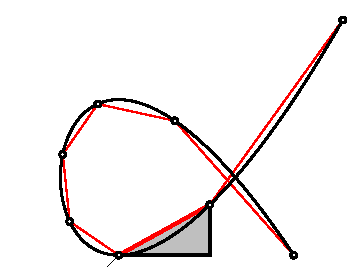
\includegraphics{09arclength.pdf}}
        \put(147.99,  10.33){\sffamily\itshape \makebox[0pt][c]{$P_0$}}
    \put( 88.63,  77.11){\sffamily\itshape \makebox[0pt][c]{$P_1$}}
    \put( 43.47,  85.90){\sffamily\itshape \makebox[0pt][c]{$P_2$}}
    \put( 48.60,  -8.73){\sffamily\itshape \makebox[0pt][c]{$P_{k-1}$}}
    \put( 96.68,  33.86){\sffamily\itshape \makebox[0pt][c]{$P_{k}$}}
    \put(166.52, 122.56){\sffamily\itshape \makebox[0pt][c]{$P_{n}$}}
    \put( 73.84,  -4.33){\sffamily\itshape $\Delta x_k$}
    \put(103.68,  15.76){\sffamily\itshape $\Delta y_k$}
    \put( 76.84,  19.76){\sffamily\itshape \makebox[0pt][r]{$\Delta s_k$}}
\end{picture}
}}
  \parbox{178pt}{{
    \begin{picture} (170.000000,128.000000)(0,0)
    \put(0.0, 0.0){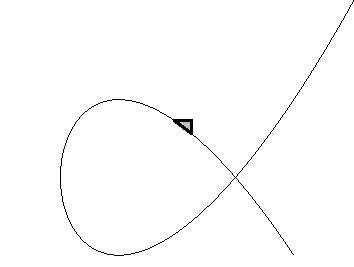
\includegraphics{09arclength-Leibniz.pdf}}
        \put( 79.88,  61.18){\sffamily\itshape $ds$}
    \put( 87.94,  73.18){\sffamily\itshape \makebox[0pt][c]{$dx$}}
    \put( 95.00,  65.09){\sffamily\itshape \makebox[0pt][l]{$dy$}}
\end{picture}
}}
  \caption{\textbf{The distance travelled. } On the left the picture describing
    the derivation with Riemann sums, on the right Leibniz' version of the
    picture.}
  \label{fig:09arclength}
\end{figure}
distance travelled by finding the length of this polygon.  The distance between
two consecutive points $P_{k-1}$ and $P_k$ is
\begin{align*}
  \Delta s_k
  &= \sqrt{(\Delta x_k)^2 + (\Delta y_k)^2}\\
  &= \sqrt{\Bigl(\frac{\Delta x_k}{\Delta t_k}\Bigr)^2 + \Bigl(\frac{\Delta
      y_k}{\Delta t_k}\Bigr)^2}
  \;\; \Delta t_k\\
  &\approx \sqrt{x'(c_k)^2 + y'(c_k)^2}\; \Delta t_k
\end{align*}
where we have approximated the difference quotients
\[
\frac{\Delta x_k}{\Delta t_k} \text{ and } \frac{\Delta y_k}{\Delta t_k}
\]
by the derivatives $x'(c_k)$ and $y'(c_k)$ for some sample time $c_k$ in the
interval $[t_{k-1}, t_k]$.

The total length of the polygon is then
\[
\sqrt{x'(c_1)^2 + y'(c_1)^2}\; \Delta t_1 \; +\; \cdots \; + \; \sqrt{x'(c_1)^2
  + y'(c_1)^2}\; \Delta t_1
\]
This is a Riemann sum for the integral $\int_{t_a}^{t_b} \sqrt{x'(t)^2 +
  y'(t)^2} \;dt$, and hence we find that the distance travelled is
\begin{equation}
  s=\int_{t_a}^{t_b} \sqrt{x'(t)^2 + y'(t)^2} \;dt.
  \label{eq:09distance-travelled}
\end{equation}

As usual, Leibniz has a shorter version of this derivation: \itshape%
during an infinitely small time interval of length $dt$, the coordinates of the
point change by $dx$ and $dy$, respectively.  The (infinitely short) distance
$ds$ travelled during this time interval follows from Pythagoras (see
Figure~\ref{fig:09arclength}), so the point moves a distance
\[
ds = \sqrt{(dx)^2 + (dy)^2} = \sqrt{\Bigl(\frac{dx}{dt}\Bigr)^2 +
  \Bigl(\frac{dy}{dt}\Bigr)^2} \; dt.
\]
The total distance travelled is the sum of all these infinitely small
displacements:
\[
s= \int_{t_a}^{t_b} ds = \int_{t_a}^{t_b} \sqrt{\Bigl(\frac{dx}{dt}\Bigr)^2 +
  \Bigl(\frac{dy}{dt}\Bigr)^2} \; dt.
\]%
\upshape%
Of course, you have to believe in infinitely small numbers when you use this
argument.

\section{The arclength of a curve} %{{{1
We introduced the integral as a tool to compute areas of plane regions.  You can
also use it to compute arclengths of plane curves.  In fact, if the curve is a
parametric curve, given by $x=x(t)$, $y=y(t)$ then we already have the formula.
The arclength of the curve traced out by the point $\bigl(x(t), y(t)\bigr)$ as the
parameter $t$ varies from $t_a$ to $t_b$ is nothing but the distance travelled
by the point.  We can use \eqref{eq:09distance-travelled} to find the length.
In this section we'll do three examples of length computations.  One point that
these examples will show is that the formula \eqref{eq:09distance-travelled}
is a good source of impossible or very difficult integrals.


\subsection{The circumference of a circle} %{{{2
You can parametrize the circle with radius $R$ by
\[
x(t) = R\cos t, \quad y(t)=R\sin t,\quad (0\leq t\leq 2\pi)
\]
The velocity is $v(t) = \sqrt{x'(t)^2+y'(t)^2} = R$.
Therefore \eqref{eq:09distance-travelled} tells us that the length of the
circle is
\marginpar{\footnotesize\input ../figures/221/09motion-on-unitcircle.pdf_tex }%
\[
L = \int_0^{2\pi}\sqrt{x'(t)^2+y'(t)^2}\;dt = \int_0^{2\pi} R\;dt = 2\pi R.
\]
The length of a circle is $2\pi R$ -- we knew that.
This cannot be a PROOF that the circle has length $2\pi R$ since we have
already used that fact to define angles in radians, to define the trig functions
sine and cosine, and to find their derivatives.  But our computation shows that
the length formula \eqref{eq:09distance-travelled} is at least consistent with
what we already knew.

\subsection{The length of the graph of a function $y=f(x)$} %{{{2
In Chapter~V, \S~\ref{sec:motion-on-a-graph}, we saw that you can parametrize
the graph of a function $y=f(x)$, by
\[
  x(t) = t, \qquad y(t) = f(t).
\]%
\marginpar{\def\svgwidth{90pt}%
\footnotesize\sffamily%
\input ../figures/221/05motion-on-a-graph.pdf_tex
}%
For such a parametric curve you have $x'(t) = 1$ and $y'(t) = t$, so the length
of the segment with $a\leq t\leq b$ is $\int_a^b \sqrt{1+f'(t)^2} dt$.  In that
integral $t$ is a dummy variable and we can replace it with $x$, which leads to
a formula for the length of the graph of a function $y=f(x)$:
\begin{equation}
  L = \int_a^b \sqrt{1+f'(x)^2}\, dx
  \label{eq:09length-of-graph-of-f}
\end{equation}

\subsection{Arclength of a parabola} %{{{2
Consider our old friend, the parabola $y=x^2$, $0\leq x\leq 1$.  While the area
under its graph was easy to compute ($\frac13$), its arclength turns out to be much
more complicated.
\marginpar{\sffamily\itshape\footnotesize\input ../figures/221/09motion-on-parabola.pdf_tex \\
Area: $1/3$\\
Length: \\
\null\hfill $\tfrac12 \sqrt{5} + \tfrac14 \ln\bigl(2+\sqrt{5}\bigr) $.}%
Our length formula \eqref{eq:09length-of-graph-of-f} says that the arclength of the
parabola is given by
\begin{equation}
  L = \int_0^1 \sqrt{1+\bigl(\frac{dx^2}{dx}\bigr)^2}\;dx =\int_0^1
  \sqrt{1+4x^2}\;dx.
  \label{eq:09length-of-parabola}
\end{equation}
To find this integral you would have to use one of the following (not at all
obvious) substitutions\footnote{Many calculus textbooks will tell you to
substitute $x = \frac12\tan\theta$, but the resulting integral is still not
easy. }
\begin{equation}
  x=\tfrac14\left(z-\frac1z\right)\qquad
  \text{(then $1+4t^2 =\frac14(z+1/z)^2 $ so
  you can simplify the $\sqrt{\cdots}$)}
  \label{eq:09rationalizing-substitution}
\end{equation}
or (if you like hyperbolic functions)
\[
  x = \tfrac12\sinh w\qquad \text{(in which case $\sqrt{1+4x^2} = \cosh w$.)}
\]
The answer is :
\[
  L = \tfrac12 \sqrt{5} + \tfrac 14 \ln\bigl(2+\sqrt{5}\bigr) \approx 1.47894\cdots
\]
The computation is left as a challenging exercise (Problem
\ref{ex:09length-of-parabola}).

\subsection{Arclength of the graph of the sine function} %{{{2
To compute the length of the curve given by $y=\sin x$, $0\leq x\leq \pi$ you
would have to compute this integral:
\begin{equation}\label{eq:09lengthOFsineGraph}
  L
  = \int_0^\pi \sqrt{1+\left(\frac{d\sin x}{dx}\right)^2}\; dx
  = \int_0^\pi \sqrt{1+\cos^2 x}\; dx.
\end{equation}%
\marginpar{\input ../figures/221/09how-long-the-sine.pdf_tex}%
Unfortunately this is not an integral that can be computed in terms of the
functions we know in this course (it's an ``elliptic integral of the second
kind.'')  This happens very often with the integrals that you run into when you
try to compute the arclength of a curve.  In spite of the fact that we get stuck
when we try to compute the integral in \eqref{eq:09lengthOFsineGraph}, the
formula is not useless.  For example, since $-1\leq \cos x\leq 1$ we know that
\[
  1\leq \sqrt{1+\cos ^2 x} \leq \sqrt{1+1} = \sqrt2,
\]
and therefore the length of the sine graph is bounded by
\[
  \int_0^\pi 1dx \;\leq\; \int_0^\pi \sqrt{1+\cos^2 x}\; dx \;\leq\;
  \int_0^\pi\sqrt2\;dx,
\]
i.e.
\[
  \pi \leq L \leq \pi\sqrt2.
\]

\begin{multicols}{2}[
\section{Problems} %{{{1
\problemfont %{{{3
]\setlength{\parindent}{0pt}

\problem The velocity of a particle moving along the $x$-axis is %{{{3
\[
  v(t)=-(t-1)^2+2
\]
for $0 \leq t \leq 6$. If at time $t=0$ the particle is at the origin, find the
location of the particle at time $t=3$.

\problem A snail travels at a constant speed of $0.001$ units per hour on a %{{{3
straight path from point $A(1,1)$ to point $B(2,3)$.

\subprob Find a parametrization of the snail's motion and use it to compute the
distance traveled by the snail.

\subprob Is there an easier way to find the distance travelled, and does it
lead to the same result?

\problem Find the length of the piece of the graph of $y=\sqrt{1-x^2}$ where %{{{3
$0\le x\le \frac12$.

The graph is a circle, so there are two ways of computing this
length.  One uses geometry (length of a circular arc $=$ radius times angle),
the other uses an integral.

Use both methods and check that you get the same answer.
\answer %{{{3
The answer is $\pi/6$.

To get this using the integral you use formula
\eqref{eq:09length-of-graph-of-f} with $f(x) = \sqrt{1-x^2}$.
You get $f'(x) = -x/\sqrt{1-x^2}$, so 
\[
\sqrt{1+f'(x)^2} = \frac{1}{\sqrt{1-x^2}}.
\]
The integral of that is $\arcsin x (+C)$, so the answer is
$\arcsin\tfrac12 - \arcsin 0 = \pi/6$.
\endanswer

\problem Compute the length of the part of the \textit{evolute of the circle}, %{{{3
given by
\[
x(t) = \cos t + t\sin t, \quad y(t) = \sin t - t\cos t
\]
where $0 \leq t \leq \pi$.
(This problem has a nice answer, but any small algebra error can lead you to an
impossible integral.)

\problem \groupproblem Show that the \textit{Archimedean spiral}, given by %{{{3
\[
x(\theta) = \theta\cos\theta, \; y(\theta) = \theta\sin\theta,\;
0\le \theta\le \pi
\]
has the same length as the parabola given by
\[
y=\tfrac12 x^2,\quad 0\le x\le \pi.
\]
Hint: you can set up integrals for both lengths.  If you get the same
integral in both cases, then you know the two curves have the same
length (even if you don't try to compute the integrals).

\problem Three equivalent problems, pick one: %{{{3

\subprob  Let $N(t)$ denote the size of a bacteria population at time $t$.  The
dynamics of the population is given by
\[
  \frac{dN}{dt}=3e^{-2t}
\]
with $N(0)=25$. Express the change in population size between time $0$ and time
$t$ as an integral.  Compute the change in population size between $t=0$ and
$t=10$.

\subprob  The amount $X(t)$ of oil spilled into the ocean waters by a faulty
ship varies in time according to the rule
\[
  \frac{dX}{dt}=3e^{-2t}.
\]
Time is measured in hours. If at time $t=0$ of the first measurement, the amount
of oil in the water was already $X(0)=25$ liters, how much oil was spilled in the
water during the first $10$ hours of measurements?

\subprob  A particle is moving along the $x$-axis with velocity $v(t)=3e^{-2t}$.
If at time $t=0$ the particle was positioned at $x=25$, what is the distance
traveled by the particle during the time interval $0 \leq t \leq 10$?

\problem A rope that hangs between two poles at $x=-\ln 2$ and $x=\ln 2$ takes %{{{3
the shape of a \textit{Catenary}, with equation
\[
  y(x)=\frac{1}{4}\bigl(e^x+e^{-x}\bigr).
\]
\subprob Find an integral for the length of the rope.

\subprob Compute the integral you got in part \textbf{(a)}.

\problem \label{ex:09length-of-parabola} %{{{3
Find the length of the parabola $L$ in \eqref{eq:09length-of-parabola}
by using the substitution \eqref{eq:09rationalizing-substitution}.
\end{multicols}
\noproblemfont
\section{Velocity from acceleration} %{{{1
The acceleration of the object is by definition the rate of change of its
velocity,
\[
a(t) = v'(t),
\]
so you have
\[
v(t) = v(0) + \int_{0}^{t} a(\bar t)d\bar t .
\]
Conclusion: \textit{If you know the acceleration $a(t)$ at all times $t$, and
  also the velocity $v(0)$ at time $t=0$, then you can compute the velocity
  $v(t)$ at all times by integrating.}

\subsection{Free fall in a constant gravitational field} %{{{2
If you drop an object then it will fall, and as it falls its velocity increases.
The object's motion is described by the fact that \textit{its acceleration is
constant}.  This constant is called $g$ and, at sea level on Earth, it is about $9.8
\textrm{m}/\textrm{sec}^2 \approx 32\textrm{ft}/\textrm{sec}^2$.  If we
designate the upward direction as positive then $v(t)$ is the upward velocity of
the object, and this velocity is actually decreasing.  Therefore the constant
acceleration is negative: it is $-g$.

If you write $h(t)$ for the height of the object at time $t$ then its velocity
is $v(t) = h'(t)$, and its acceleration is $h''(t)$.  Since the acceleration is
constant you have the following formula for the velocity at time $t$:
\[
v(t) = v(0) + \int_0^t (-g)\; d\bar t = v(0)-gt.
\]
Here $v(0)$ is the velocity at time $t=0$ (the ``initial velocity'').  To get
the height of the object at any time $t$ you must integrate the velocity:
\marginpar{\footnotesize%
\input ../figures/221/09falling-cars.pdf_tex}
\begin{align*}
  h(t) &= h(0) + \int_{0}^t v(\bar t)\;d\bar t
  &&\text{(Note the use of the dummy $\bar t$)}\\
  &=h(0) + \int_0^t \bigl[v(0) - g \bar t\bigr]\;d\bar t
  &&\text{(use $v(\bar t) = v(0)-g\bar t$)}\\
  &=h(0) + \bigl[v(0)\bar t -\tfrac12 g \bar t^2\bigr]_{\bar t=0}^{\bar t=t}\\
  &=h(0) + v(0) t -\tfrac12gt^2.
\end{align*}

For instance, if you launch the object upwards with velocity
$5\textrm{ft}/\textrm{sec}$ from a height of $10\textrm{ft}$, then you have
\[
h(0) = 10\textrm{ft},\quad v(0) = +5\textrm{ft}/\textrm{sec},
\]
and thus
\[
h(t) = 10 + 5t-32t^2/2 = 10+5t-16t^2.
\]
The object reaches its maximum height when $h(t)$ has a maximum, which is when
$h'(t)=0$.  To find that height you compute $h'(t) = 5-32t$ and conclude that
$h(t)$ is maximal at $t=\frac{5}{32}\textrm{sec}$.  The maximal height is then
\[
h_{\textrm{max}} = h(\tfrac5{32}) = 10+\tfrac{25}{32}-\tfrac{25}{64}=
10\tfrac{25}{64}\textrm{ft}.
\]



\section{Work done by a force} %{{{1

\subsection{Work as an integral} %{{{2
According to  Newtonian mechanics any force that acts on an object in motion
performs a certain amount of work, i.e.\ it transfers a certain amount of
energy.  (In Physics ``work'' is a form of energy.)
\begin{center}
  \small\sffamily\itshape%
  \input ../figures/221/09work.pdf_tex 
\end{center}

If the acting force is constant then the work done by this force is
\[
\hbox{Work} \;=\; \hbox{Force}\;\cdot\;\hbox{Distance of displacement}.
\]
For example, if you are pushing a box forward then there will be two forces
acting on the box: the force you apply, and the friction force of the floor on
the box. The amount of work you do is the product of the force you exert and the
length of the displacement.  Both displacement and the force you apply are
pointed towards the right, so both are positive, and the work you do (energy you
provide to the box) is positive.

The amount of work done by the friction is similarly the product of the friction
force and the displacement.  Here the displacement is still to the right, but
the friction force points to the left, so it is negative.  The work done by the
friction force is therefore negative.

Suppose now that the force $F(t)$ on the box is not constant, and that its
motion is described by saying that its position at time $t$ is $x(t)$.  The
basic formula $\textit{work} = \textit{force}\cdot\textit{displacement}$ does
not apply directly since it assumes that the force is constant.  To compute the
work done by the varying force $F(t)$ during some time interval $t_a < t < t_b$,
we partition the time interval into lots of short intervals, 
\[
t_a = t_0 < t_1< \cdots < t_{N-1} < t_N = t_b.
\]
In each short time interval $t_{k-1}\leq t\leq t_k$ we assume the force is
(almost) constant and we approximate it by $F(c_k)$ for some sample time
$t_{k-1}\leq c_k\leq t_k$.  If we also assume that the velocity $v(t) = x'(t)$
is approximately constant between times $t_{k-1}$ and $t_k$ then the
displacement during this time interval will be
\[
x(t_k)-x(t_{k-1}) \approx v(c_k) \Delta t_k,
\]
where $\Delta t_k = t_k-t_{k-1}$.  Therefore the work done by the force $F$
during the time interval $t_{k-1}\leq t\leq t_k$ is
\[
\Delta W_k = F(c_k)v(c_k)\Delta t_k.
\]
Adding the work done during each time interval we get the total work done by the
force between time $t_a$ and $t_b$:
\[
W = F(c_1)v(c_1)\Delta t_1 + \cdots + F(c_N)v(c_N)\Delta t_N.
\]
Again we have a Riemann sum for an integral.  If we take the limit over finer
and finer partitions we therefore find that the work done by the force $F(t)$ on
an object whose motion is described by $x(t)$ is
\begin{equation}
  \label{eq:work-done-by-F}
  W = \int_{t_a}^{t_b} F(t) v(t) dt,
\end{equation}
in which $v(t) = x'(t)$ is the velocity of the object.

\subsection{Kinetic energy} %{{{2
Newton's famous law relating force and acceleration says
\[
  F=ma.
\]
In this formula, $F$ is the sum of all the forces exerted on some object and 
$m$ is its mass, and $a$ is the acceleration of the object.
For instance, in the box example above, $F$ is the sum of $F_{\sf push}$ and
$F_{\sf friction}$.  Newton's law predicts that if the pushing force and the
friction force don't cancel precisely, then its velocity must be changing.

If the position of the object at time $t$ is $x(t)$, then its velocity and
acceleration are $v(t) = x'(t)$ and $a(t) = v'(t) = x''(t)$, and thus the total
force acting on the object is
\[
F(t) = ma(t) = m \frac{dv}{dt}.
\]
The work done by the total force is therefore
\begin{equation}
  \label{eq:09work-is-change-in-kinetic-E}
  W = \int_{t_a}^{t_b} F(t)v(t)dt
  =\int_{t_a}^{t_b} m \frac{dv(t)}{dt}\;v(t)\;dt.
\end{equation}
Even though we have not assumed anything about the motion, so we don't know
anything about the velocity $v(t)$, we can still do this integral.  The key is
to notice that, by the chain rule,
\[
m \frac{dv(t)}{dt}\;v(t) = \frac{d}{dt}\left[\frac12m v(t)^2\right].
\]
(Remember that $m$ is a constant.)  This says that the quantity
\[
K(t) = \tfrac12 m v(t)^2
\]
is the antiderivative we need to do the integral
\eqref{eq:09work-is-change-in-kinetic-E}.  We get
\[
W = \int_{t_a}^{t_b} m \frac{dv(t)}{dt}\;v(t)\;dt = \int_{t_a}^{t_b} K'(t)\;dt
=K(t_b) - K(t_a).
\]
In Newtonian mechanics the quantity $K(t)$ is called \emph{the kinetic energy}
of the object, and our computation shows that \textit{the amount by which the
kinetic energy of an object increases is equal to the amount of work done on
the object. }

\section{Problems} %{{{1
\problemfont %{{{3
\begin{multicols}{2}

\problem A ball is thrown upward from a height of $6$ ft, with an initial velocity of $32$ ft/sec. Is %{{{3
that enough speed for the ball to clear a fence $17$ ft high?

\problem A particle with mass $m$ on a straight line (the $x$-axis) is being %{{{3
pushed and pulled by a force of magnitude $F(t) = F_0 \sin (\omega t)$.  Here
$F_0$ is the amplitude of the force, and $\omega$ is the frequency at which it
oscillates.  $m$, $F_0$, and $\omega$ are constants.

\subprob What is the acceleration of the particle?
If the initial velocity was $v_0$, and if the particle starts at $x=0$, then where is
the particle at time $t$?

\subprob What effect does an increase in the frequency $\omega$ have on the
velocity $v(t)$ of the particle?

\problem Give a shorter derivation \textit{a la } Leibniz of the integral for %{{{3
work in equation \eqref{eq:work-done-by-F}.

\problem As an object falls, the force of gravitation transfers energy to the %{{{3
object.  Let $h(t)$ be the height of the object at time $t$.  

\subprob Use the integral \eqref{eq:work-done-by-F}, i.e.
\[
  W = \int_{t_a}^{t_b} Fv\,dt
\]
to show that the work done by gravitation during a time interval $t_a < t< t_b$
is
\[
  W = -mg\bigl(h_b - h_a\bigr),
\]
where $h_a = h(t_a)$ and $h_b = h(t_b)$.

(Hint:  $v(t) = \frac{dh}{dt}$.)

\subprob If you throw a ball in the air, and catch it when it returns to the
same height, how much work did the gravitational force do on the ball?

\problem (\textit{Rocket Science}.) %{{{3
A rocket is shot straight up into space.  Its height, measured from the
center of the Earth, is $r(t)$.  The gravitational force on the rocket gets less
as it gets further away from the Earth.  According to another of Newton's laws
the force is
\[
  F_{\sf grav} = -mg \frac{R^2}{r(t)^2},
\]
where $m$ is the mass of the rocket, $g=9.81\textrm{m}/\textrm{sec}^2$, and
$R$ is the radius of the Earth.

If the rocket starts at radius $R$ (the Earth's surface) and ends at radius
$2R$, how much work did the gravitational force apply to the rocket?
Use \eqref{eq:work-done-by-F} again.  In this problem $v = \frac{dr}{dt}$.

\begin{center}
  \input ../figures/221/09once-the-rockets-are-up.pdf_tex
\end{center}

\end{multicols}



%%% Local Variables: 
%%% mode: latex
%%% TeX-master: "free221"
%%% TeX-engine: xetex
%%% End: 
